

The pinching effect can be observed when
two functions without a
perfect match are aligned, taking the $\mathbb{L}^2$ distance as energy.
To minimize the
energy term $E$ in eqn. \ref{EQ:ENERGY}, the optimal solution will tend to squeeze
a region whose features make it difficult to align, until it disappears. Figure \ref{FIG:PINCHING}
shows the pinching effect on the registration of two functions.
A part of $f_2$ is identical to $f_1$ over [0, 0.6] and completely different
over the remaining domain. The optimal solution will tend to squeeze the second
part of $f_2$, until it vanishes completely.

\begin{figure}[Pinching force effect]{FIG:PINCHING}{Pinching force effect}
	\subfigure[SBFIG:PINCHING1]{ $f_1$ and $f_2$}{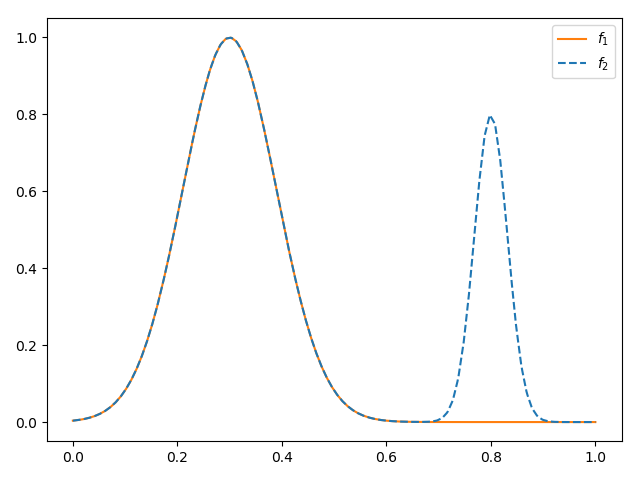
\includegraphics[width=7.5cm]{pinching-dataset}} \quad
	\subfigure[SBFIG:PINCHING2]{Pinching effect}{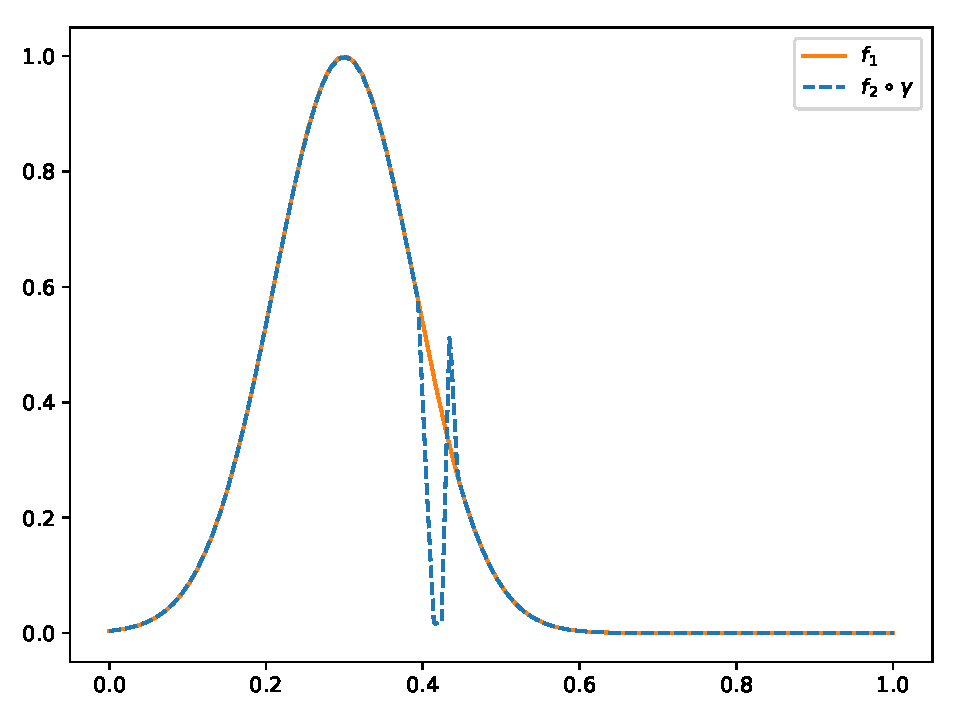
\includegraphics[width=7.5cm]{pinching-effect}}
\end{figure}
